\chapter{Aeronautical limitation surfaces}
	\section{Physical limitation surfaces}
	\paragraph{} In order to calculate all the limitation surfaces, the \cite{Standards2016} has been followed. In this document, all the limitation surfaces are fully defined following the restrictions and recommendations given for each. Furthermore, there is also a little explanation of each limitation surface, how does it work and how has to be referenced. Its important to remember that the surfaces have to be empty of any possible object in order to guarantee the correct function of the airport and the maximum security for the air plane crew and the passengers. The following to images will be attached in order to ease the understanding of the limitation surfaces and their objective:
	
	\begin{figure}[H]
		\centering
		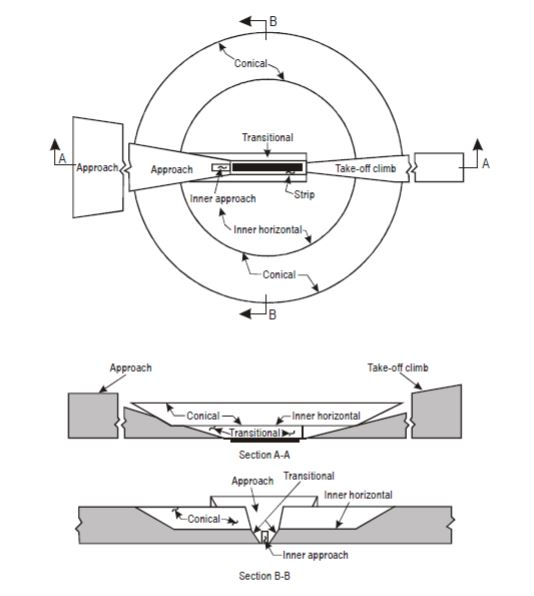
\includegraphics[clip, trim=0cm 0cm 0cm 0cm, width=0.60\textwidth]{./images/servidumbres/servidumbres}
		\caption{2D Obstacle Limitation Surface model.}
		\label{}
	\end{figure}
	 
	 Due to the fact that a general view of all the limitation surfaces doesn't allow us to have a lot of detail of the inner ones, the following image shows limitation surfaces closest to the runway and the terminal.
	 
	 \begin{figure}[H]
	 	\centering
	 	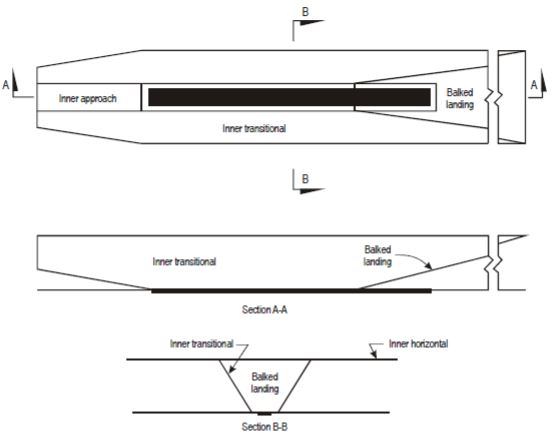
\includegraphics[clip, trim=0cm 0cm 0cm 0cm, width=0.7\textwidth]{./images/servidumbres/servidumbres2}
	 	\caption{Inner approach, inner transitional and balked landing obstacle limitation surfaces.}
	 	\label{}
	 \end{figure}
	
	Now that a general idea about the limitation surfaces have been given, the next step is to follow the table taken form the ICAO's Annex in order to calculate and obtain the final values of each surface in case of approach:
	
	\begin{figure}[H]
		\centering
		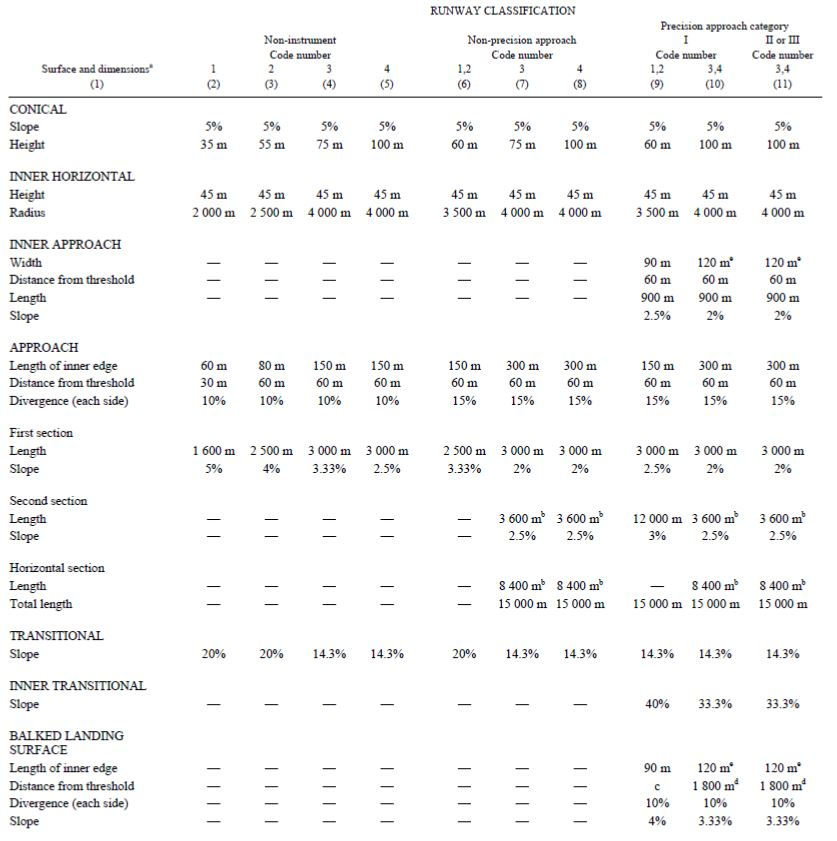
\includegraphics[clip, trim=0cm 0cm 0cm 0cm, width=1\textwidth]{./images/servidumbres/taula}
		\caption{Dimensions and slopes of obstacle limitation surfaces.}
		\label{}
	\end{figure}

	This table takes into account all the limitation surfaces considered in the approach and landing performance, thus, due to the fact that both runways will also handle takeoff performances, there is the need of an extra limitation surface. The following table gathers all the parameters needed in order to calculate and define the takeoff limitation surface:
	
	\begin{figure}[H]
		\centering
		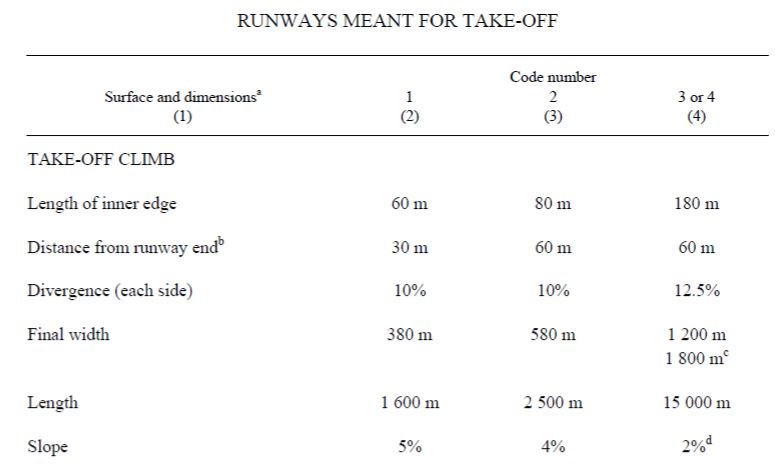
\includegraphics[clip, trim=0cm 0cm 0cm 0cm, width=0.85\textwidth]{./images/servidumbres/taulatakeoff}
		\caption{Dimension and slope of takeoff obstacle limitation surface.}
		\label{}
	\end{figure}
	